% ****** Start of file aipsamp.tex ******
\documentclass[%
 aip,
 jmp,%
 amsmath,amssymb,
%preprint,%
 reprint,%
%author-year,%
%author-numerical,%
]{revtex4-2}
\usepackage{subfigure}
\usepackage{graphicx}% Include figure files
\usepackage{dcolumn}% Align table columns on decimal point
\usepackage{bm}% bold math
%\usepackage[mathlines]{lineno}% Enable numbering of text and display math
%\linenumbers\relax % Commence numbering lines

\begin{document}

\preprint{AIP/123-QED}

\title[Catalytic knowledge graph construction and application]{Catalytic knowledge graph construction and application}% Force line breaks with \\
\thanks{Footnote to title of article.}

\author{Qingqing Li}
\altaffiliation{Chemistry and Chemical engineering Department, Xiamen University.}%Lines break automatically or can be forced with \\
\email{liqingqing@stu.xmu.edu.cn}

\date{\today}% It is always \today, today,
             %  but any date may be explicitly specified

\begin{abstract}
Relay catalysis is an important method to synthesize main chemicals for material design. But the 
the current implementation of relay catalysis remains in the traditional time-consuming 
and labor-intensive paradigm. To facilitate this process, we try to build an automatic natural language 
processing pipeline to extract reaction information from articles, constructing a reaction 
database with a knowledge graph for relay catalysis to support specific-product synthesis pathway selection/design or other applications.

.
%
\end{abstract}

\keywords{Knowledge graph, Relay catalysis, Reaction database, Specific-product synthesis pathway selection}%Use the show keys class option if the keyword
                              %display desired
\maketitle

% \begin{quotation}
% The ``lead paragraph'' is encapsulated with the \LaTeX\ 
% \verb+quotation+ environment and is formatted as a single paragraph before the first section heading. 
% (The \verb+quotation+ environment reverts to its usual meaning after the first sectioning command.) 
% Note that numbered references are allowed in the lead paragraph.
% %
% The lead paragraph will only be found in an article being prepared for the journal \textit{Chaos}.
% \end{quotation}


\section{Introduction}


\subsection{Relay catalysis}

The traditional catalytic model refers to one catalyst catalyzing one reaction, 
synthesizing the target product through a step-by-step synthesis in a linear fashion.
However, modern organic synthesis advocates atomic economy and economy of steps.
Relay catalysis can combine multiple catalysts to achieve a one-pot tandem reaction,
which can dramatically reduce waste, solvents, time, labor, etc, and can be well controlled. 
It is a perfect way to synthesize compounds we need and is more in line with green 
chemistry guidelines and modern organic synthesis requirements. Therefore, 
relay catalysis is an essential method for the fabrication of key chemicals
such as ethanol and formaldehyde. Nevertheless, the current implementation of 
relay catalysis, such as the selection of synthesis pathways from syngas to ethanol, 
remains in the traditional paradigm of a time-consuming and labor-intensive manual 
search for reactions based on experience and extensive literature reading. Therefore, 
we would like to have a reaction database that stores a large amount of reaction information, 
which can support us in implementing functions such as synthesis path design/selection 
and help us to find a high-selectivity and low-energy pathway to obtain the target product.


\subsection{Reaction database}
To this end, we investigated existing reaction databases(Table \ref{table.1}) and found that they 
all focused on the storage of organic reactions, mostly manually constructed and not easily
accessible for commercial or other reasons. In addition, Pistachio and the USPTO dataset are derived from patent data without real-time effects,
while Scifinder and Reaxys store reaction information in an unstructured manner. Besides, all of the 
above are relational databases that do not have inference capabilities. Therefore, the construction 
of a database for relay-catalyzed reactions became necessary.


\begin{table}[h!]
\begin{tabular}{ |p{3cm}|p{3cm}|p{3cm}|p{3cm}|p{3cm}|  }
\hline
Database&Developer&Method&Focus&Avaliability\\ \hline
CAS data(SciFinder)& ACS    &Manually curated&   Organic reactions&Not avaliable\\ \hline
Reaxys&   Elsevier  & Manually curated   &Organic reactions&For commercial use\\ \hline
Pistachio & NextMove & Java-based extraction &  Organic reactions&Not avaliable\\ \hline
AZ ELN(AstraZeneca ELN)    &AstraZeneca & Manually curated&  Organic reactions&Not avaliable\\ \hline
USPTO&   Daniel Lowe  & Java-based extraction&Organic reactions&Only <2016 avaliable\\ \hline
ORD(open reaction database) & MIT and Google  & Manually curated   &Organic or Inorganic reactions&Avaliable but manually upload\\ \hline
\end{tabular}
\caption{Existing reaction databases}
\label{table.1}
\end{table}

\subsection{Knowledge graph}

In recent years, with the development of artificial intelligence, the knowledge graph has gradually 
attracted our attention. It is a multivariate relational graph where nodes represent entities and 
edges represent relationships between entities. In a knowledge graph, a triple is used to represent a 
fact such as Einstein was born in the German Empire in a subject-verb-object structure, and then 
these triples are associated to form the structure of the graph(Fig \ref{ Fig.2 }).
As knowledge graphs can easily represent different types of data, facilitate path queries and can support inference, 
and prediction tasks, It is used by many platforms as a base data support such as DBpedia, Freebase, Wikidata,
YAGO, etc. In recent years it has also been used in materials science to assist in materials design, 
so we choose the knowledge graph as the underlying data structure for the Relay Catalysis database, aiming to build a catalytic reactions knowledge base.

\begin{figure}[htbp]
 \centering
 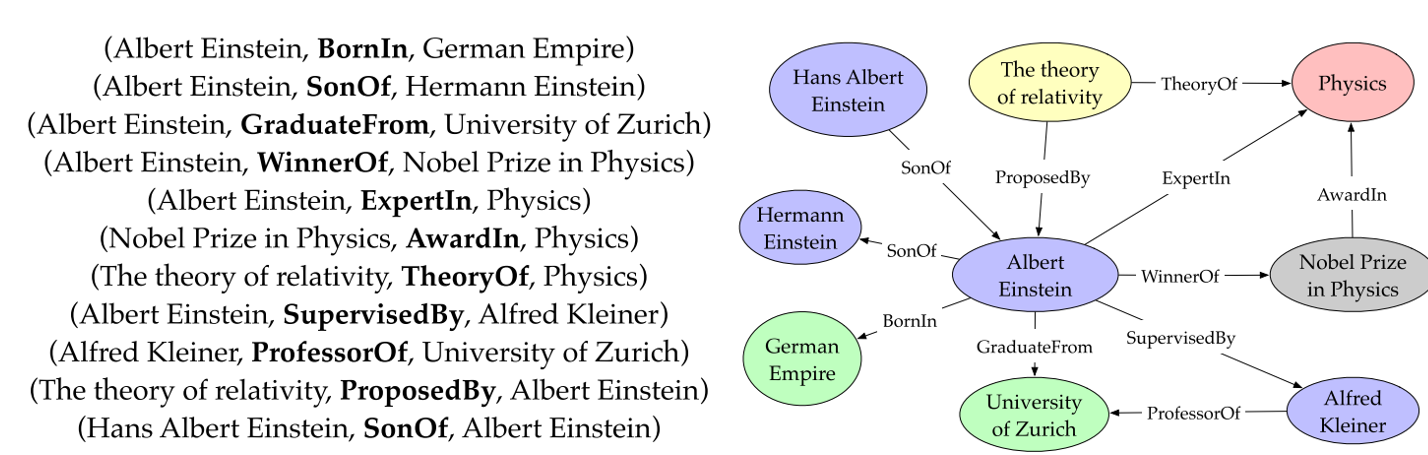
\includegraphics[width=0.7\textwidth]{figure/2.png}
 \caption{ An example of knowledge graph }
 \label{ Fig.2 }
\end{figure}

The process of building a knowledge graph starts from the raw data and uses a series of automated or 
semi-automated technical means to extract knowledge elements (facts) from the raw data and store them 
in the data and schema layers of the knowledge base. It is an iterative updating process and according 
to the logic of knowledge acquisition, each iteration consists of three stages: information extraction, 
knowledge fusion and knowledge processing(Fig \ref{ Fig.1 }). Information extraction, that is, to extract 
entities, attributes and the relationship between entities from various types of data sources, 
such as that we can extract Steve Balmer, Microsoft, as entities, and CEO as a relation between these entities from
the text (Steve Balmer, the CEO of Microsoft). Knowledge fusion, after acquiring new knowledge, needs to be 
integrated to eliminate contradictions and ambiguities. For example, some entities may have multiple 
expressions, and a particular title may correspond to many different entities. Like the Seattle-headquartered 
the software giant and the richest man in the world both refer to Bill Gates. In knowledge processing, for the integrated new knowledge, 
we can construct ontology and conduct knowledge reasoning to gain more knowledge elements (facts) making the knowledge graph complete. 

\begin{figure}[htbp]
 \centering
 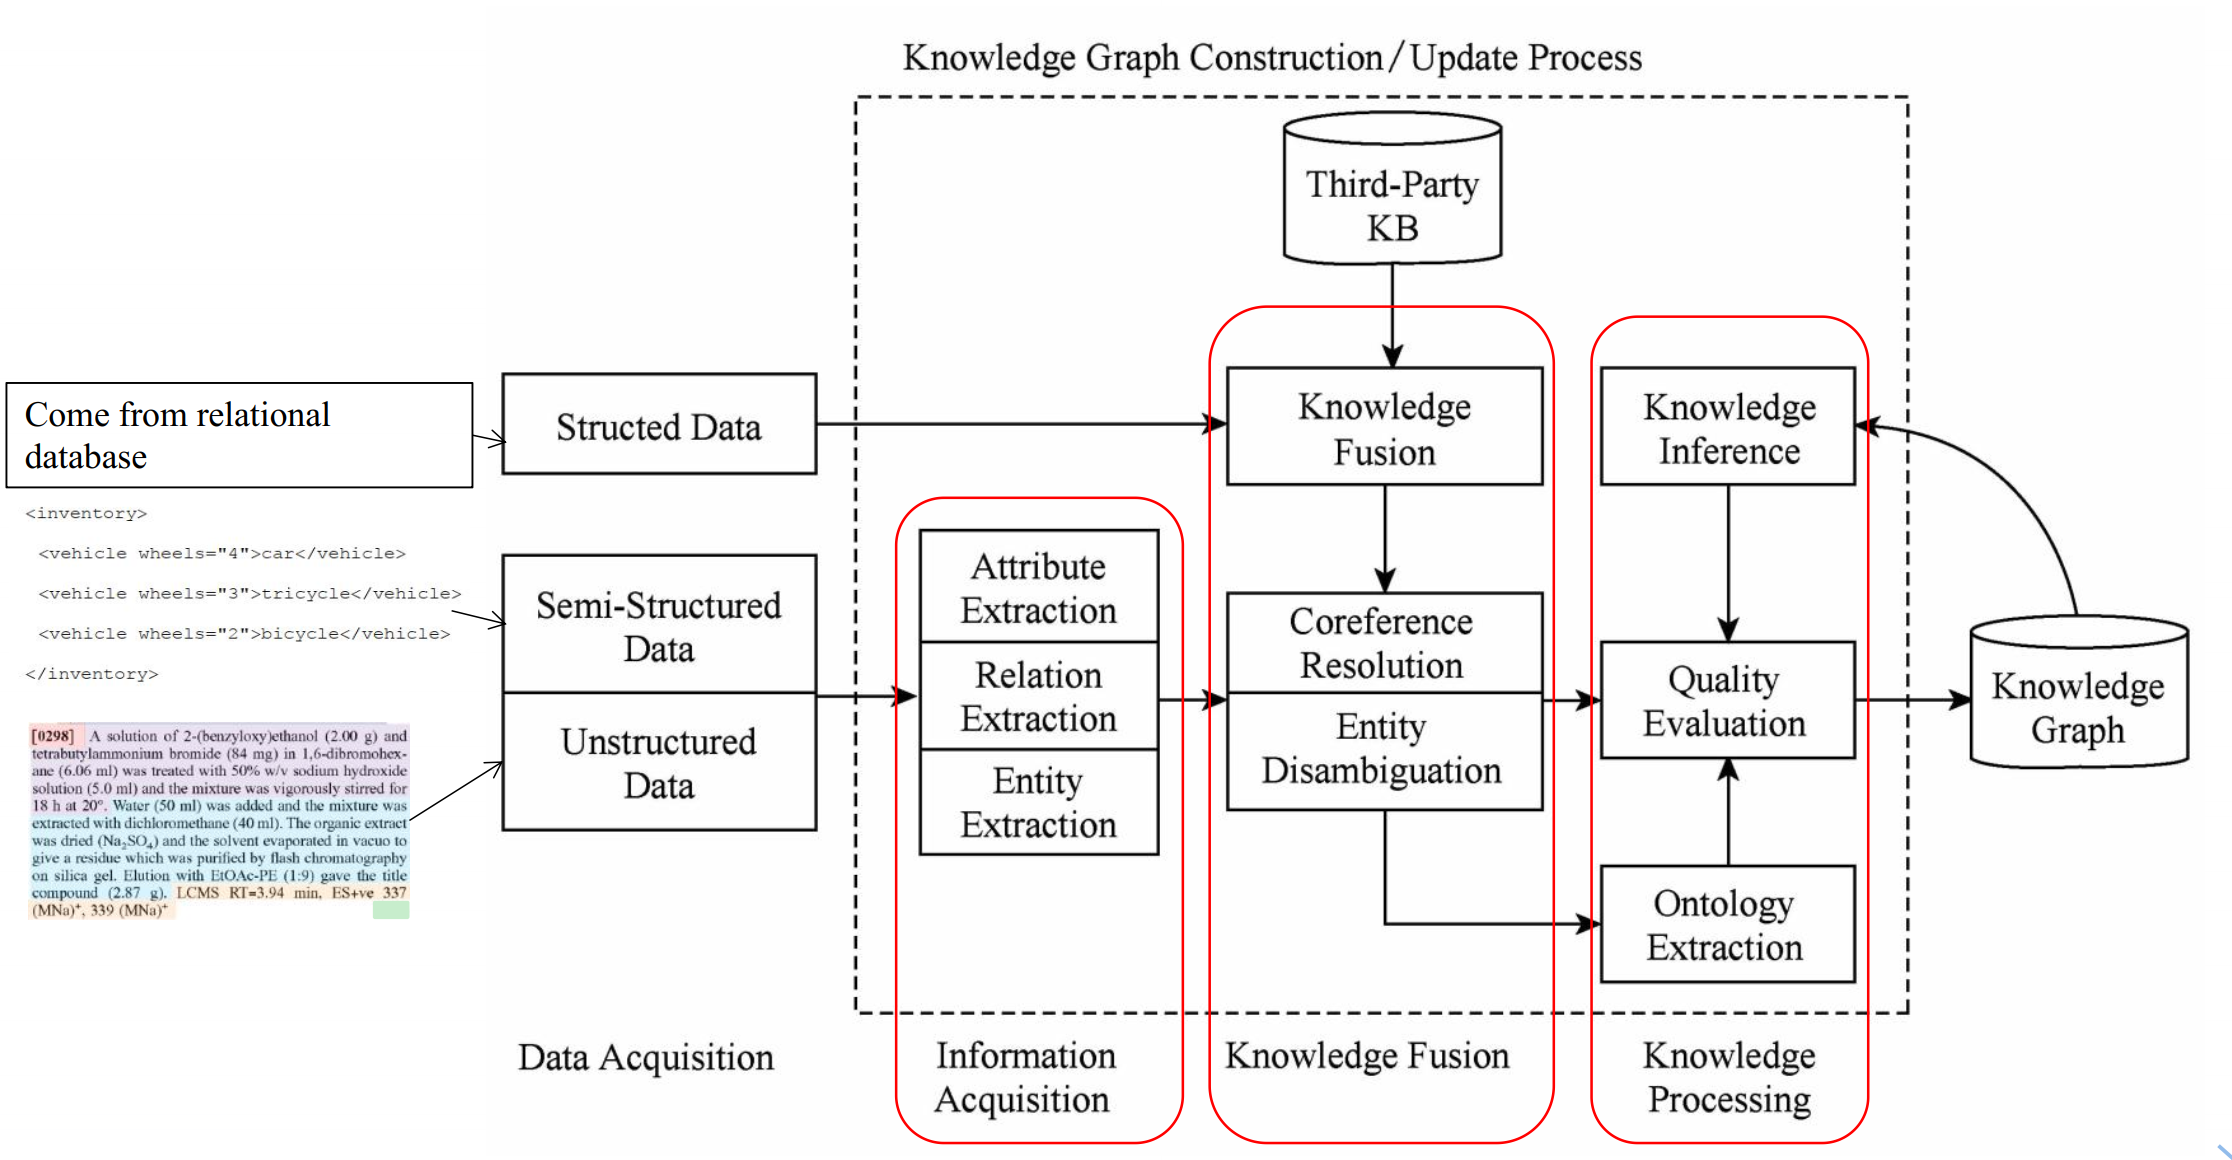
\includegraphics[width=0.7\textwidth]{figure/1.png}
 \caption{ Construction of a knowledge graph }
 \label{ Fig.1 }
\end{figure}

To construct a knowledge graph for a specific domain, in our work, this domain refers to chemistry, we can generally divide the graph 
construction into two parts-a schemas, which describes the concepts in the domain and the relationships 
between these concepts, e.g. redox reactions are a subclass of reaction, such data patterns are stored and 
managed by an ontology library, and a data layer, which stores specific data such as the 
product of react:face is acetophenone(Fig \ref{ Fig.3 }). The construction of the data layer actually 
corresponds to the extraction of reaction information, and the schema layer corresponds 
to the construction of ontology. 

\begin{figure}[htbp]
 \centering
 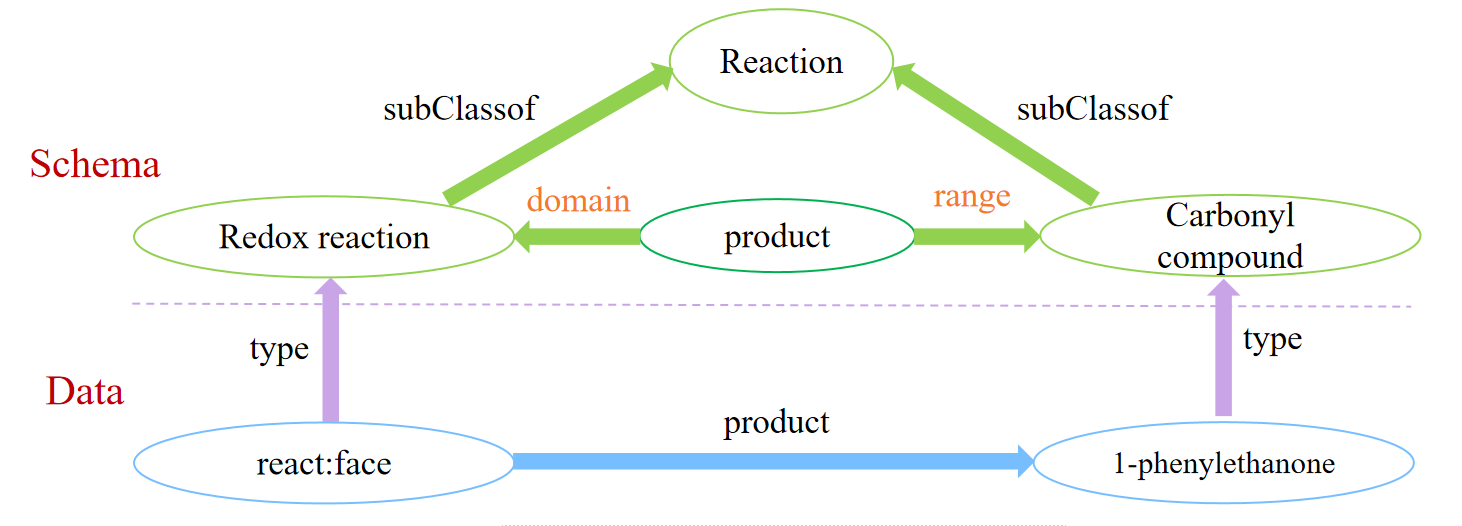
\includegraphics[width=0.7\textwidth]{figure/3.png}
 \caption{ Schema layer and data layer of a knowledge graph }
 \label{ Fig.3 }
\end{figure}

\section{Research condition}




\section{Related work}
We investigated four specific research directions of reaction extraction-entity recognition, relation extraction
and reaction extraction with these methods.

\subsection{Entity recognition}
Entity recognition refers to detecting named entities from text and classifying them into predefined classes.
In general, existing methods can be divided into the rule-based method, statistical model-based approach and 
deep learning-based approach.
% Rule-based approach
The rule-based approach is the early method of writing hand-curated rules, such as regular matching, curated 
by specialists of a specific domain. This extraction style can achieve
high accuracy and recall when it is used on small datasets. However, as the dataset grows, 
the rule-set construction cycle becomes longer and less flexible.
% Statistical model-based approach
The statistical model-based approach train model with a completely annotated corpus or partially annotated corpus.
The main models used are Hidden Markov Model, Conditional Markov Model, Maximum Entropy Model and Conditional Random
Fields Model. These methods regard entity recognition as a sequence-to-sequence problem.
% Deep learning-based approach
With the widespread adoption of deep learning methods in the field 
of natural language processing, the deep neural network is applied to 
entity recognition with good effects. In contrast to traditional 
statistical models, deep learning-based approaches take a vector of words in the text as input directly and implement end-to-end named entity recognition through neural networks, no longer relying on manually defined features.
Currently, neural networks used for named entity
recognition are Convolutional Neural networks (CNN), 
Recurrent Neural networks (RNN) and neural networks 
that introduces the Attention Mechanism. In general, the different
neural network structures act as encoders in the named entity 
recognition process, obtaining a new vector representation 
of each word based on the initial input and the contextual 
information of the word, and finally outputting the annotation 
results for each word through a CRF model.
% Chemical entity recognition
The emergence of "big data" initiatives has led to the need for tools that 
can automatically extract valuable information from large volumes of unstructured
data, such as the scientific literature. Since chemical information can be present
in figures, tables, and textual paragraphs, successful information extraction often
depends on the ability to interpret all of these domains simultaneously. A complete
toolkit is present for the automated extraction of chemical entities and their associated
properties, measurements, and relationships from scientific documents that can be used
to populate structure chemical databases. It uses unsupervised word clustering based on
a massive corpus of chemistry  articles to achieve chemical named entity recognition with an 
F-score of 93.4%.

\subsection{Relation extraction}
Relation extraction is one of the most important sub-tasks of knowledge extraction for 
unstructured text data, where the semantic relationship between two or more entities is extracted 
from the text. Relation extraction is closely related to entity extraction, generally after 
identifying the entities in the text, then extracting the possible relationships between them, 
or many joint models do both tasks together. The following are some of the main methods
for extracting relations.

\subsubsection{Templete-based approach}
For the text "water is a reactant of WGS reaction", the pattern can be constructed as "[1] is a reactant of [2]",
We can get entities for "is a reactant of" relation with this pattern. The advantage of the template-based relationship 
extraction approach is that templates are simple to construct and allow relatively quick implementation of relationship 
extraction systems on small datasets. Similarly, when the data size is large, manual construction of templates takes 
a lot of time for domain experts. In addition, template-based relationship extraction systems are less portable, 
requiring the templates to be rebuilt when faced with the same problem in another domain. 
Finally, the recall rate of template-based relationship extraction systems is generally low due to 
the limited number of manually constructed templates and the insufficient coverage of templates.

\subsubsection{Supervised learning-based approach}
Supervised learning-based relationship extraction methods transform relationship extraction into a classification 
problem by training a supervised learning model for relationship extraction based on a large amount of annotated 
data. The general steps in relationship extraction using supervised learning methods include: predefining the 
type of relationship; manually annotating the data; designing the features required for relationship recognition 
(relying on feature engineering), which are typically computed based on the context of the sentence 
in which the entity is located; selecting a classification model (e.g. support vector machines, 
neural networks and plain Bayes) and training the model based on the annotated data; 
and evaluating the trained model.

\subsubsection{Deep learning-based approach}
At present, existing deep learning-based relation extraction methods can be divided into two classes:
pipelined method and joint extraction method.
The pipeline method treats entity recognition and relation extraction as two separate processes that 
do not affect each other, but the relation extraction task is performed based on results of entity recognition,
therefore, the results of relation extraction rely on that of entity extraction such as CR-CNN,
Att-Pooling-CNNs and Att-BLSTM.These methods have the following disadvantages:
\begin{itemize}
    \item[1] Error propagation, where errors in the entity recognition module affect the performance of the following relation extraction.
    \item[2] Ignoring the relation between the two subtasks.
    \item[3] Unnecessary redundant information is generated as the identified entities are paired in pairs and then classified relationally, those unrelated entity pairs introduce redundant information and raise the error rate.
\end{itemize}
Joint extraction methods combine entity extraction and relation extraction, where a sentence is an input 
and a triplet of entities with relations is directly obtained by a joint model of entity recognition 
and relation extraction. This can overcome the drawbacks of the pipelined approach above, but probably cause more 
complex structures such as BERT, LSTM-RNN, DGCNN, etc.

\subsubsection{weakly supervised learning-based approach}
Supervised learning-based relationship extraction methods require a large training corpus, 
especially for deep learning-based methods, where the optimization of the model relies more on a 
large amount of training data. When the training corpus is insufficient, weakly supervised learning methods 
can use only a small amount of annotated data for model learning. Weakly supervised learning-based relationship 
extraction methods mainly include remotely supervised methods and Bootstrapping methods.

% remotely supervised methods
The remotely supervised approach automatically constructs a large amount of training data by 
aligning the knowledge graph with unstructured text, reducing the model's reliance on manually 
annotated data and enhancing the model's cross-domain adaptability. The underlying assumption 
of the remotely supervised approach is that if two entities have some relationship in the knowledge graph, 
then the sentences containing both entities express that relationship. The remotely supervised relation 
extraction method can make use of the rich knowledge graph information to obtain training data, 
effectively reducing the workload of manual annotation. However, based on the assumption of 
remote supervision, a large amount of noise will be introduced into the training data, 
thus triggering the phenomenon of semantic drift. Existing work includes PCNNs (Piecewise Convolutional Neural Networks) and
CNN-RL.

% Bootstrapping methods
The Bootstrapping method originates from the autonomous sampling method in statistics, 
which uses a small number of instances as an initial seed set, then learns on the seed set 
to obtain a template for relationship extraction, and then uses the template to extract more instances 
to be added to the seed set. Through continuous iteration, the Bootstrapping method can extract 
a large number of instances of a relationship from the text. Several entity relationship extraction 
systems use the Bootstrapping approach, such as DIPER, Snowball and NELL, but they are out-update. 
The advantages of the Bootstrapping approach are that the relationship extraction system is cheap to build, 
suitable for large-scale relationship extraction tasks, and can discover new relationships. 
However, the sensitivity to initial seeds, the problem of semantic drift and the low accuracy of the 
results have made the bootstrapping method fade out of the limelight.

\subsection{Reaction extraction}
There are some works about extracting reaction information from texts.

Daniel Lowe download patent data from USPTO as an extraction source and use machine learning and rule-based 
methods to extract reaction information into a representation containing atomic position information, 
but this approach has two shortcomings, one being that the patent data does not provide a good picture 
of trends in the field of chemical synthesis, and the rule-based extraction of reactions results in 
low accuracy and low recall information.

To solve these two problems Regina Barzelay's team at the MIT Computer Science and Artificial Intelligence Laboratory published a work 
in 2021 that structured the reaction information into eight fields including product, reaction type, reactant, solvent, etc. Using a 
natural language processing approach, the reaction information extraction process was divided into two parts, entity identification tasks
with reaction products as a central element and other elements that will be related to the product and do the relation extraction task.
Implementing the conversion of a piece of text into a structured response message. For such work, it costs tens of students to label sentences
from articles, spend more than 200 hours to label and check the accuracy of labeling work, which is time-consuming and labor-intensive.

Weiren Wang proposed a natural language processing pipeline to capture both chemical composition and property data from articles that allow analysis
and prediction of superalloys. It uses a heuristic text multiple-relation extraction distance-based algorithm to get properties without any labeled samples.
which can easily solve the above problem.

\subsection{Atom-Atom mapping}
For applications like verifying the correctness of a reaction, template-based reaction prediction, 
retrosynthesis planning methods, reactant-reagent role assignments, reaction rules extraction and knowledge
extraction from reaction databases. To verify the correctness of a reaction refers to a reaction must have 
at least one product and two reactants/solvents/catalysts,reactants and products do not have the same structures,
for a correct reaction, all atoms of the product must come from the reactants and the number of atoms of the
reactants and the number of atoms of the products should be the same in the calculation.After the information on 
the reaction has been correctly extracted, in order to be able to achieve the above applications.It is necessary
to know how atoms are converted during a reaction, a process we call atomic mapping.To automate this process, 
IBM's European Research Institute Philip's team co-sourced the atomic mapping tool called RXNMapper 
in 2021.Supports the conversion of Smiles representation into Smiles representation with 
corresponding atomic positions, and atomic mapping for different types of reactions, 
with a combined mapping accuracy of 99.4%.

\subsection{Ontology construction}
Ontologies are used to define concepts in a particular domain and the relationships between concepts. They serve two purposes: to constrain 
the data and to facilitate knowledge graph queries.Since the various compounds in chemistry are more clearly defined and related to each other.
Ontologies can be built in a top-down seven-step process(Fig \ref{ Fig.4 }), which is simply divided 
into reusing existing ontologies and building custom ontologies using build tools.
\begin{figure}[htbp]
 \centering
 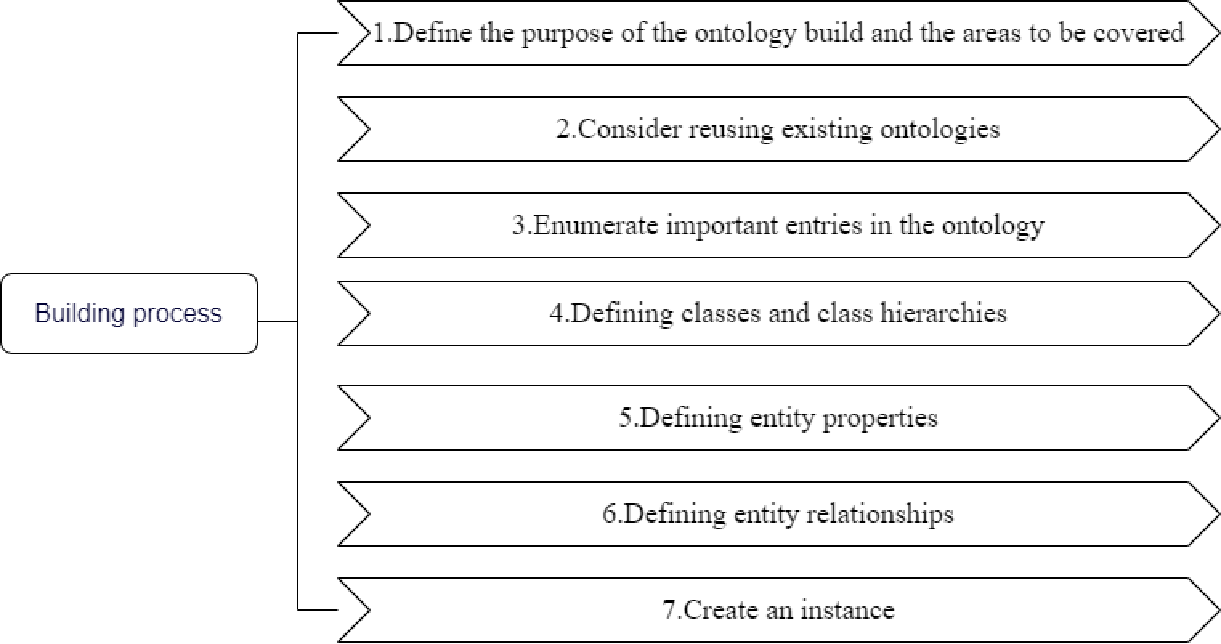
\includegraphics[width=0.7\textwidth]{figure/4.png}
 \caption{ A top-down seven-step process of building an ontology }
 \label{ Fig.4 }
\end{figure}

ChEBI is a database of compounds published in 2007 by the Institute of Bioinformatics-Kirill team at the University of Cambridge that 
describes small molecule compounds in biochemistry using standard bioinformatics terminology, providing compound names, structures, 
descriptors and ontology information.Here is the ontological structure of cobalt in CHEBI and the relationship between a cobalt atom, 
a metal atom, and a metal atom.Due to its organic and inorganic content and clear structure, the ZOOMA tool provides the possibility 
of converting chemical names in the text into ontology corresponding categories to be used as the basic ontology of the catalytic 
knowledge base in relation to specific data.For categories that cannot be represented by the basic ontology, the semi-automated ontology 
building tool Protege can be used to build the relevant concepts and relationships on its own, thus completing the construction of the 
schema layer.

\section{work foundation}
In order to build the Relay Catalytic Knowledge Map, the following preparations have been made.

\subsection{Schema design}
A catalytic reaction message is expressed as 30 fields containing reactants, products, catalysts, reaction conditions, etc(Fig \ref{ Fig.5 }). as follows:
\begin{figure}[htbp]
 \centering
 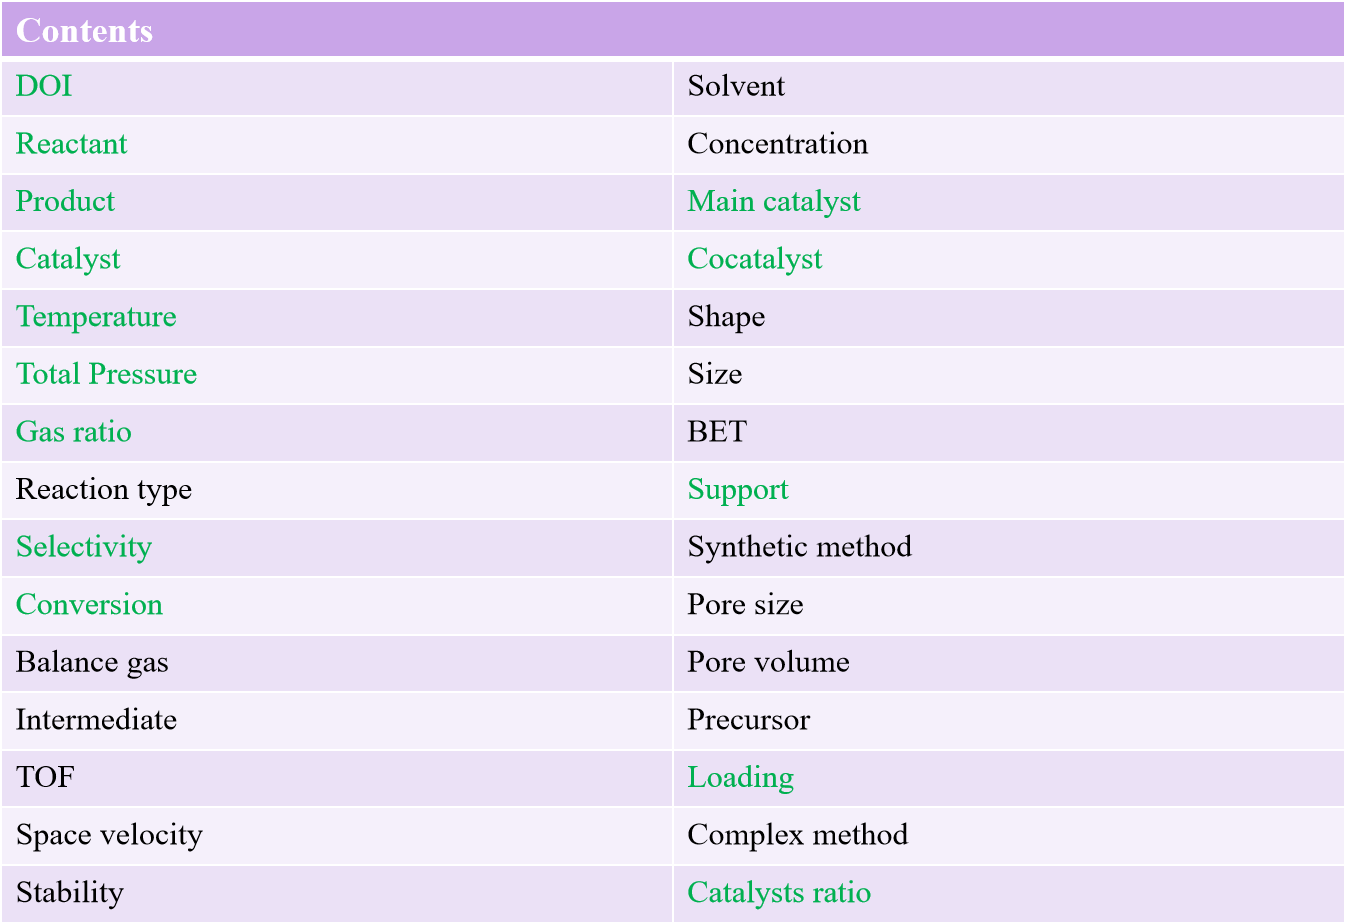
\includegraphics[width=0.7\textwidth]{figure/5.png}
 \caption{ Schema of one reaction }
 \label{ Fig.5 }
\end{figure}
\subsection{Article collection}
A total of over 10,000 papers were then collected using these keywords from the following publishers' journals(Fig \ref{ Fig.6 }).
\begin{figure}[htbp]
 \centering
 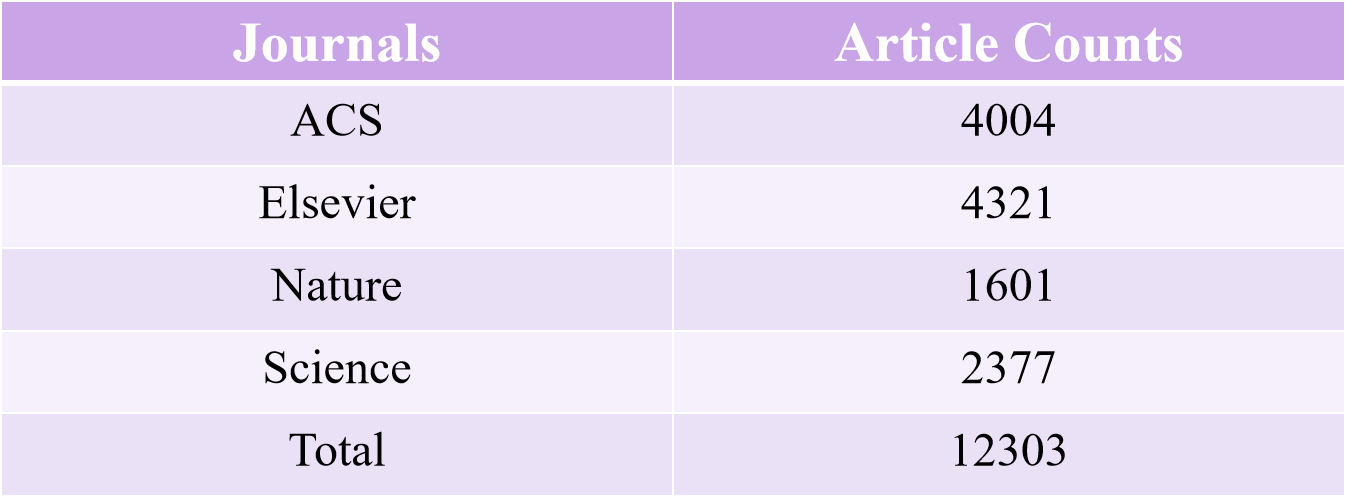
\includegraphics[width=0.7\textwidth]{figure/6.png}
 \caption{ Number of Articles per Journal in Our Corpus }
 \label{ Fig.6 }
\end{figure}
\subsection{Reaction extraction}
To extract reactions from articles, we try to divide the extraction task into two parts, one is reaction extraction from text, 
another is reaction extraction from tables.To achieve reaction extraction from text, we first need to know if current paragraph
contains the target reaction information or not.
% 训练词向量
we try to use the total 12303 articles to train word vector preparing for text classification.
% 尝试段落分类
Use trained word vector to get paragraph text vector and apply to SVM, Random Forest method to classify paragraph.
% 尝试规则提取化合物与属性
If current paragraph contains the target reaction information, then input it into rule-based or NLP method to extract
chemicals and properties.
% 尝试表格提取化合物及属性
Tables as semi-structured data, can be easily extracted from articles.we use Beautifulsoup to extract tables in articles as lists,
then use tailored algorithms to extract reaction information from these lists. 
After extraction from text and tables, we can combine these information to make reaction complete.

\section{summary}
We plan to automate the process of extracting information from documents to structured reactions(Fig \ref{ Fig.7 }), 
converting the structured information into a knowledge graph through existing tools. It is hoped that such knowledge 
mapping can be applied to scenarios such as synthesis path
selection, reaction result prediction, reaction innovation, checking the correctness of reactions, and experimental condition screening.
\begin{figure}[htbp]
 \centering
 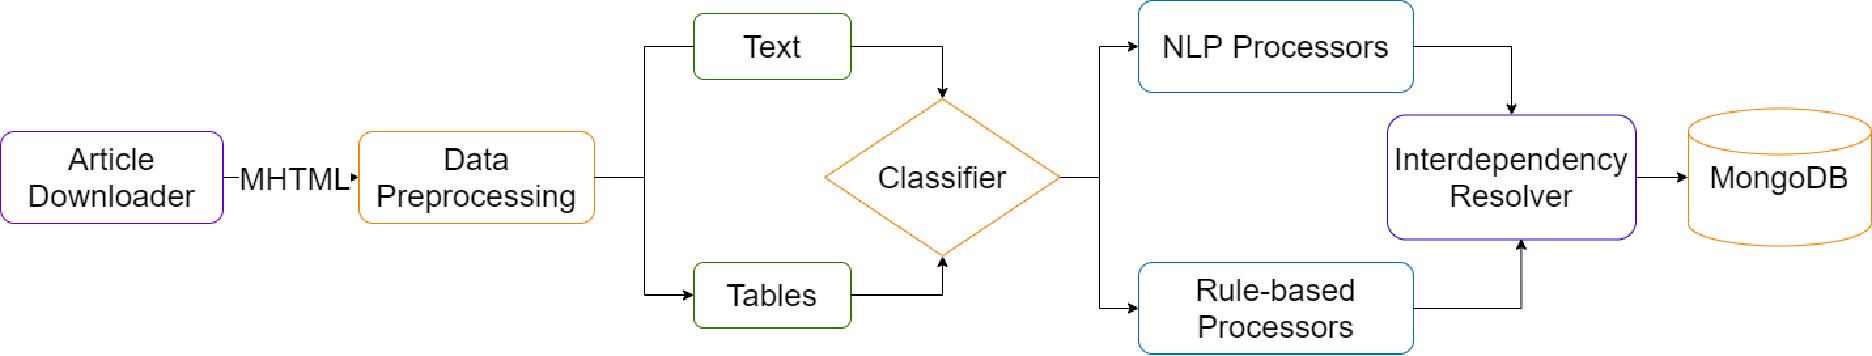
\includegraphics[width=0.7\textwidth]{figure/7.png}
 \caption{ Flowchart of reaction extraction }
 \label{ Fig.7 }
\end{figure}
The current research work has several challenges, based on the fragmentation of information, the need to do document-level information 
integration, and the need to map referents to specific entities. Some attributes appear in sentences in the form of phrases that cannot 
be simply extracted by rules, and need to be combined with natural language processing methods for entity recognition and relationship 
recognition. For existing specific response types, further extraction of hierarchical structures is needed when building ontologies to 
facilitate later knowledge graph searches, and this work needs to be done by domain experts, which is very time-consuming.

\begin{acknowledgments}
We wish to acknowledge the support of the author community in using
REV\TeX{}, offering suggestions and encouragement, testing new versions,
\dots.
\end{acknowledgments}

\nocite{*}
\bibliography{aipsamp}% Produces the bibliography via BibTeX.

\end{document}
%
% ****** End of file aipsamp.tex ******
